\chapter{Implementation}
\label{chapter:Chapter 4}
\lhead{Chapter 4. \emph{Implementation}}

In this Chapter, we present a description of the Implementation of \todo[inline]{need a framework name}. Firstly, we provide a Data Analysis from the provided Historical data, which \todo[inline]{needs way more talk}.

\section{Data Analysis}
\label{section: Data Analysis}
In order to gain insight and find the limitations of the AIS Data, we decided analyze the provided Historical AIS Data. For this Section, the Data Analysis we used the historical AIS Data-Set made publicly available by \cite{DATASET}.

Analysis of the provided Historical Data, was conducted by firstly analyzing the overall distribution of the Data-Set and after the analysis of each variable. 
The used Data-Set is composed of \textbf{18.684.115} AIS Messages originated by \textbf{4555} different Vessels. The Data-Set covers a Period of 6 Months (from 2015-10-01 to 2016-03-31), from a area nearby Brest, France represented in Figure \ref{fig:DS_Sample}.

\begin{figure}[H]
	\centering
	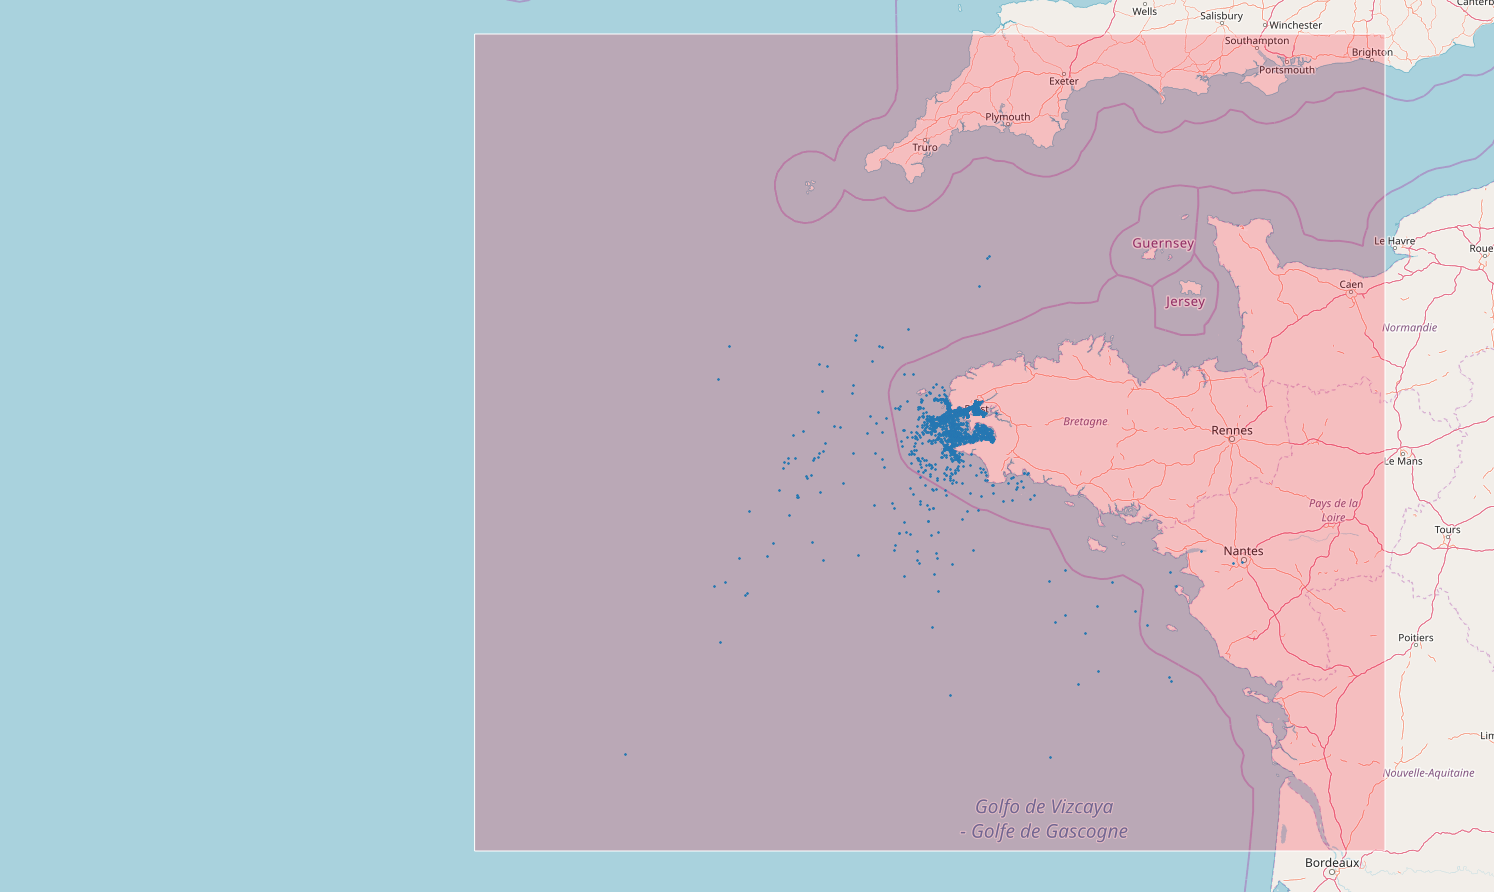
\includegraphics[scale = .23]{figures/Ch4/nari_DS_ex2.png}
    \caption{Area of the Data-Set represented in the Red, with a sample of 50.000 AIS Positions.}
    \label{fig:DS_Sample}
\end{figure}
Every AIS Message provided in the Data-Set, is composed by the features that derive from the AIS Dynamic Information. In Table \ref{Table: Data-Set Features}, we describe the Data-Set features and also the unit and range of each feature. 

\begin{table}[H]
\centering
\caption{My caption}
\label{Table: Data-Set Features}
\begin{tabular}{@{}llll@{}}
\toprule
Feature & Description                  & Unit               & Range          \\ \midrule
MMSI    & AIS Navigational Status.     &                    & 0 to 99999     \\
Status  & AIS Navigational Status.     &                    & 0 to 15        \\
Turn    & Rate of turn, right or left. & degrees per minute & 0 to 720       \\
SOG     & Speed Over Ground.           & knots              & 0 to 111*      \\
COG     & Course Over Ground.          & degrees            & 0º to 360º     \\
X       & Longitude.                   & degrees            & -180º to +180º \\
Y       & Latitude.                    & degrees            & -90º to 90º    \\
Time    & received Time-Stamp.         & Unix Time          &                \\ \bottomrule
\end{tabular}
\end{table}

With the same Data-Set it is possible to enrich the AIS Dynamic messages, with the Vessels Static information. By interpolating the MMSI we accessed information of the actual Vessels Static information, which represents the actual Vessel Characteristics, such as the dimensions of the Vessel, and what had more importance for us the Vessel Type.




posiextrapolate Vessels Static information, thus gaining information of the Vessel Characteristics, such as, the dimension characteristics of the Vessel and the Vessel type information. Vessel Type is a good indicator to filter the Data, based on the Vessel data thus knowing if

effective way, to query the Dtafilter the Vessel activities based on the Vessel type.
represented in Table, is significant to gain information by know in

\P
As any 

\todo[inline]{MORE TEXT HERE} The features represented above, were al contained 

Working with big ... INTRO

Our first cleani

\section{Implemented Framework}

\todo[inline]{need to intro the framework talk about the used techinques. -> kafka -> spark -> cassandra}

\section{Data Ingestion}

\section{Data Pre-processing}
Data Pre-processing, represents the module that handles the Raw AIS data, and Cleans Transforms and Normalizes every AIS messages, coming from the Data Ingestion Module. Each AIS message is transformed into our normalized representation of and AIS message, which we defined as a \textbf{Behavioural Point}. A Behavioural Point is a multidimensional point $Mp_{MMSI}$ is defined as:
\[Mp_{MMSI} = [t, x, y, SoG, CoG, NS]\]
Where the dimensions of the multidimensional points represent the (Time, Longitude, Latitude, Speed Over Ground, Course Over Ground and Navigational Status) respectively, a representation of these features is provided in Table 
\ref{Table: Data-Set Features}.

\subsection{Data Cleansing}
Data Cleaning refers to the process of cleaning the Data which is wrongly defined or, has wrong types. When handling with sensor Data that is transmitted is common that wrong readings occur. In AIS data, this errors tend to occur as AIS features that are not transmitted with values that don't correspond to the Feature value range. An example of this is having a Latitude being broadcast with values of 500.

For the messages transmitted with features that didn't correspond to the value range of the specific Feature, we discarded this messages. The features value range considered for the whole framework was the one presented in \ref{Table: Data-Set Features}.

\section{Feature Engineering}
\subsection{Vessel Type}
Vessel Type, is a classification system, where each Vessel is categorized by the type of activities it preforms. Classified by a numeric scale from 0 to 99; the first digit represents the general category of the subject Vessel, and the combination of the first digit with the second represent a specific activity of the Vessel. In Table XX we present the Vessel General category associated with the first digit, and also the specific Categories which are more representative in the Data-Set.

\begin{table}[H]
\centering
\caption{My caption}
\label{my-label}
\begin{tabular}{@{}llll@{}}
\toprule
First Digit & General Category & Relevant Categories &                                                                                         \\ \midrule
1           & Reserved         &                     &                                                                                         \\
2           & Wing In Ground   &                     &                                                                                         \\
3           & Special Category & 30 - Fishing        & 30 - 286(6\%)                                                                           \\
4           & High-Speed Craft &                     &                                                                                         \\
5           & Special Category &                     &                                                                                         \\
6           & Passenger        &                     &                                                                                         \\
7           & Cargo            & 70 - Cargo          & \begin{tabular}[c]{@{}l@{}}70 - 1511(33\%)\\ 79 - 273(6\%)\\ 71 - 217(5\%)\end{tabular} \\
8           & Tanker           & 80 - Tanker         & 80 - 342(7\%)                                                                           \\
9           & Other            &                     & 99 - 1192(26\%)                                                                         \\ \bottomrule
\end{tabular}
\end{table}

For the Data-Set described above in Section XX, the Static Vessel Information is available for all the Vessel in the Data-Set. Allthough, when handling Real-Time NMEA streams or other Batches of Data, the Vessel Static information is not available or broadcasted. This, creates a problem of not having the Vessel Type information which is used to query our Trajectory Data-Base.
For this we developed a \textbf{Web Scrapping application}, described in the following subsection.

\subsubsection{Web Scrapping Application}
Web Scrapping is used to extract information from freely available websites. For the sole purpose of this work, we developed an application that would retrieve the Vessel Type information from a well Known Vessel Traffic Webpage.
By giving a Vessel Identifier (MMSI) to the Vessel Type Scrapper, we retrieve the html webpage data that contains all the Vessel Information from the well Known Vessel Trafic Webpage. From the html data we, strip the html tags thus retreiving the Vessel Type Information, as it is presented in Fig. XX.


\begin{figure}[H]
	\centering
	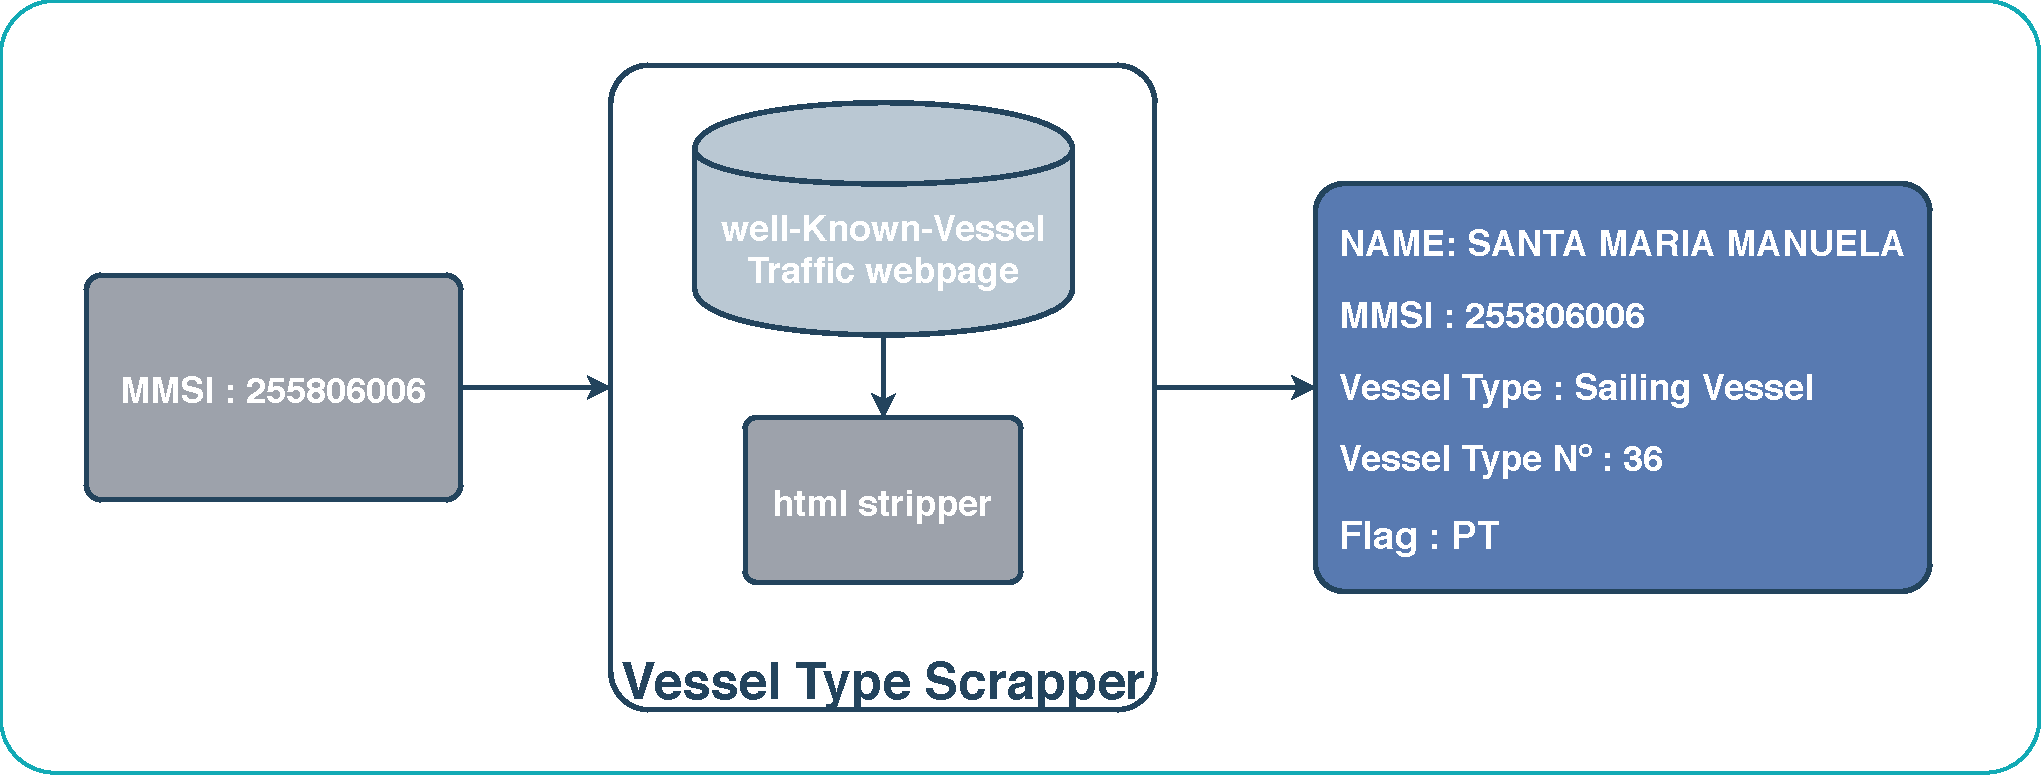
\includegraphics[scale = .4]{figures/Ch4/scrapper}
    \caption{Example of the Vessel Type Scrapper retreived information for Vessel MMSI: 255806006}
    \label{fig:DSSSSS}
\end{figure}


\subsection{Latitude Longitude Normalization}
In order to normalize the reported AIS positions, either from the AIS streams or the used Data-Set, we defined a set number of decimal cases used. This is done as most of AIS providers only assure a GPS precision of 0.0001 minutes accuracy, but what we found was that some reported positions come with up to 8 decimal cases, which can be caused just from how the Data-Set files were written.

So our normalization process, was to assure that every Vessel position was normalized to a precision on 4 decimal cases; as it represents a global position precision of 11m to 4m, as it is shown in Table \ref{Table: Degree Precision}.

\begin{table}[H]
\centering
\caption{Degree precision versus the approximate radius of measured error.}
\label{Table: Degree Precision}
\begin{tabular}{lrrrr}
\hline
\multicolumn{1}{c}{\begin{tabular}[c]{@{}c@{}}Decimal \\ Places\end{tabular}} & \multicolumn{1}{c}{Degrees} & \multicolumn{1}{c}{\begin{tabular}[c]{@{}c@{}}Precision \\ Equator\end{tabular}} & \multicolumn{1}{c}{\begin{tabular}[c]{@{}c@{}}Precision \\ 45º N/S\end{tabular}} & \multicolumn{1}{c}{\begin{tabular}[c]{@{}c@{}}Precision \\ 67º N/S\end{tabular}} \\ \hline
0 & 1.0 & 111.3Km & 78.7Km & 43.5Km \\
1 & 0.1 & 11.3Km & 7.8Km & 4.4Km \\
2 & 0.01 & 1.13Km & 787.1m & 435m \\
3 & 0.001 & 111.3m & 78.7m & 43.5m \\
4 & 0.0001 & 11.3m & 7.8m & 4.4m \\
5 & 0.00001 & 1.3m & 0.7m & 0.4m \\ \hline
\end{tabular}
\end{table}

\todo[inline]{Geohash - https://en.wikipedia.org/wiki/Geohash}



\subsection{Distance to Coast}
The Distance to Shore influences, the navigational behaviour for some type of Vessels. In order to enrich the features used in our Anomaly Detection methods it seemed necessary to extrapolate the Distance to Shore for every point in the Data-Set. Although in order to calculate the Distance to Shore over the whole data-set, and in real time to streams of AIS data it is mandatory to represent the Coastline in a efficient manner. 
For this we used the ocean coastline data\footnote{http://www.naturalearthdata.com}, which represented the Global Ocean Coast line in a vector of \textbf{547.503} points, which is equivalent of representing in a 1:10m scale.

The calculation of the closest point was done with a Nearest Neighbor approach, using the Ball Tree algorithm. The choice of this algorithm was done, due to the high volume of data we were using, and the possibility of using the Haversine Distance measures \eqref{eq: Haversine} in the already implemented methods from \todo{http://scikit-learn.org/stable/modules/generated/sklearn.neighbors.BallTree.html}.

Haversine is a distance metric commonly used in Vessel Navigation, it is commonly used as both Latitude and Longitude features are represented in a spherical coordinate system. $d_({p_1}, {p_2})$ represents the distance between the 2 point $p1(lat_1, lon_1)$ and $p2(lat_2, lon_2)$, and where $r$ represents the approximate radius of the Earth which we considered \textbf{6.367.000m} in our experiments.

\begin{equation}
d = 2r sin ^{-1} (\sqrt{sin^2(\frac{lat_{2}-lat_{1}}{2})+cos(lat_{1})cos(lat_{2})sin^2(\frac{long_{2}-long_{1}}{2}))}
\label{eq: Haversine}
\end{equation}

\subsubsection{Distance to Port}
Do i want to talk about this? Linear is not a good aproximation.

\subsection{Stopped/Moving}
Enriching the reported Vessel Kinematics by determining if whether a Vessel is Moving or Stopped represents a information gain on overall Vessel Trajectory that can be addressed, for the understanding of the normal Vessels Behaviour itself and even further, the possible detection of Anomalies.
Thus, the approaches we used to classify every Vessel transmission as Stopped or Moving is shown in the following subsections:

\textbf{Rule Based Approach}:
This approach is vastly used in the literature, as it is the simplest way to characterize the stopping of a Vessel, based solely on the Speed or as reported in the AIS the Speed Over Ground (SOG). Thus, Vessels Positions that have a Speed under a certain defined threshold $\Delta$ are considered as Stopped and the opposite are considered Moving, as it is shown in equation \ref{eq: MovingRule}, where $p_n$ represents actual point we want to the point which we want to c.
\begin{equation}
kinematic status(p_n) = \left\{\begin{matrix}
p_n.SOG > \Delta; & Moving\\ 
p_n.SOG \leq  \Delta; & Stopped
\end{matrix}\right.
\label{eq: MovingRule}
\end{equation}

The most commonly used value, found in the literature for $\Delta$ was 0.5 knots, which was also the Threshold we initially tested for, but we found that this leads to the miss-labeling of effectively Positions that are Moving, more specifically Fishing Vessels that due to their type of fishing activities, greatly slow their Speed for short periods of Time, which cannot be labeled as Stopped.
\todo[inline]{Need intro to this image}
\missingfigure{Trajectory of a Shipping Vessel that is considered as stopped.}

In order to mitigate the problem described above we used a \textbf{Rolling Mean}, which is a common method for Time Series Analysis in countless different fields.  By Smoothing the Vessels Speed Feature, we reduce the random or abrupt variations in the observed Speed features,  thus better describing the normal kinematic, stopping  pattern of a Vessel. 
\todo[inline]{Need intro to this image}
\missingfigure{Trajectory of a Shipping Vessel that is considered as stopped then with the rolling mean!}

\section{Trajectory Definition}
In this Section we present our definition our interpretation and formulation of Vessel Trajectory, 
Representing a Vessel Trajectory data, can become a difficulty in the Maritime domain. Currently there are a vast number of solutions described in the literature, presenting different solutions for different types of problems. 

Our approach to represent a Maritime trajectory, was to consider a trajectory as a whole, this is, as Vessel are obliged to broadcast their AIS information in a semi-continuous rates; knowing that each AIS broadcast message represent the instantaneous kinematic information from a Single Vessel, aggregating this information over time will represent a Vessel Trajectory. 

Thus, by identifying each vessel by its unique identifier (MMSI), the trajectory can be considered as the set of AIS messages, identified by the MMSI of each Vessel.

\begin{figure}[H]
	\centering
	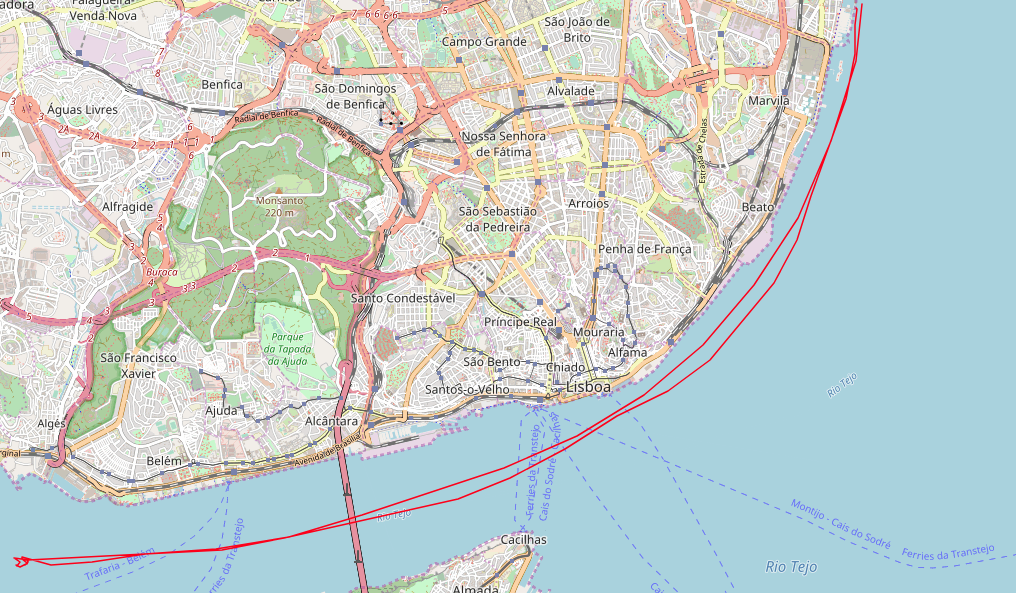
\includegraphics[scale = .3]{figures/Ch3/traj_example.png}
    \caption{Trajectory snapshot(2017-11-05 10:22 to 2017-11-05 22:42) from Vessel MMSI: 255806006}
    \label{fig: TrajectorySMM_example}
\end{figure}

Although, as each AIS message is time-stamped(contains the time in which was broadcast), our representation of trajectory can be defined as Multivariate Time-Series, this is for each trajectory we have $N$ time-series, in which $N$ represents the number of features considered for each trajectory, further explained in the subsections bellow.

\subsection{Multivariate Time-Series Analogy}
As mentioned above, each Trajectory is considered as a Time Series composed of Multiple features.  

in Fig. \ref{fig: MTimeSeries_example}, we represent the Vessel trajectory showend in figure X. 
For each trajectory we consider the features representing 
main features that a which in order to normalize our analysis of a Vessel Route, we ...
\todo[inline]{TODO dar palha para introduzir esta imagem}

\begin{figure}[H]
	\centering
	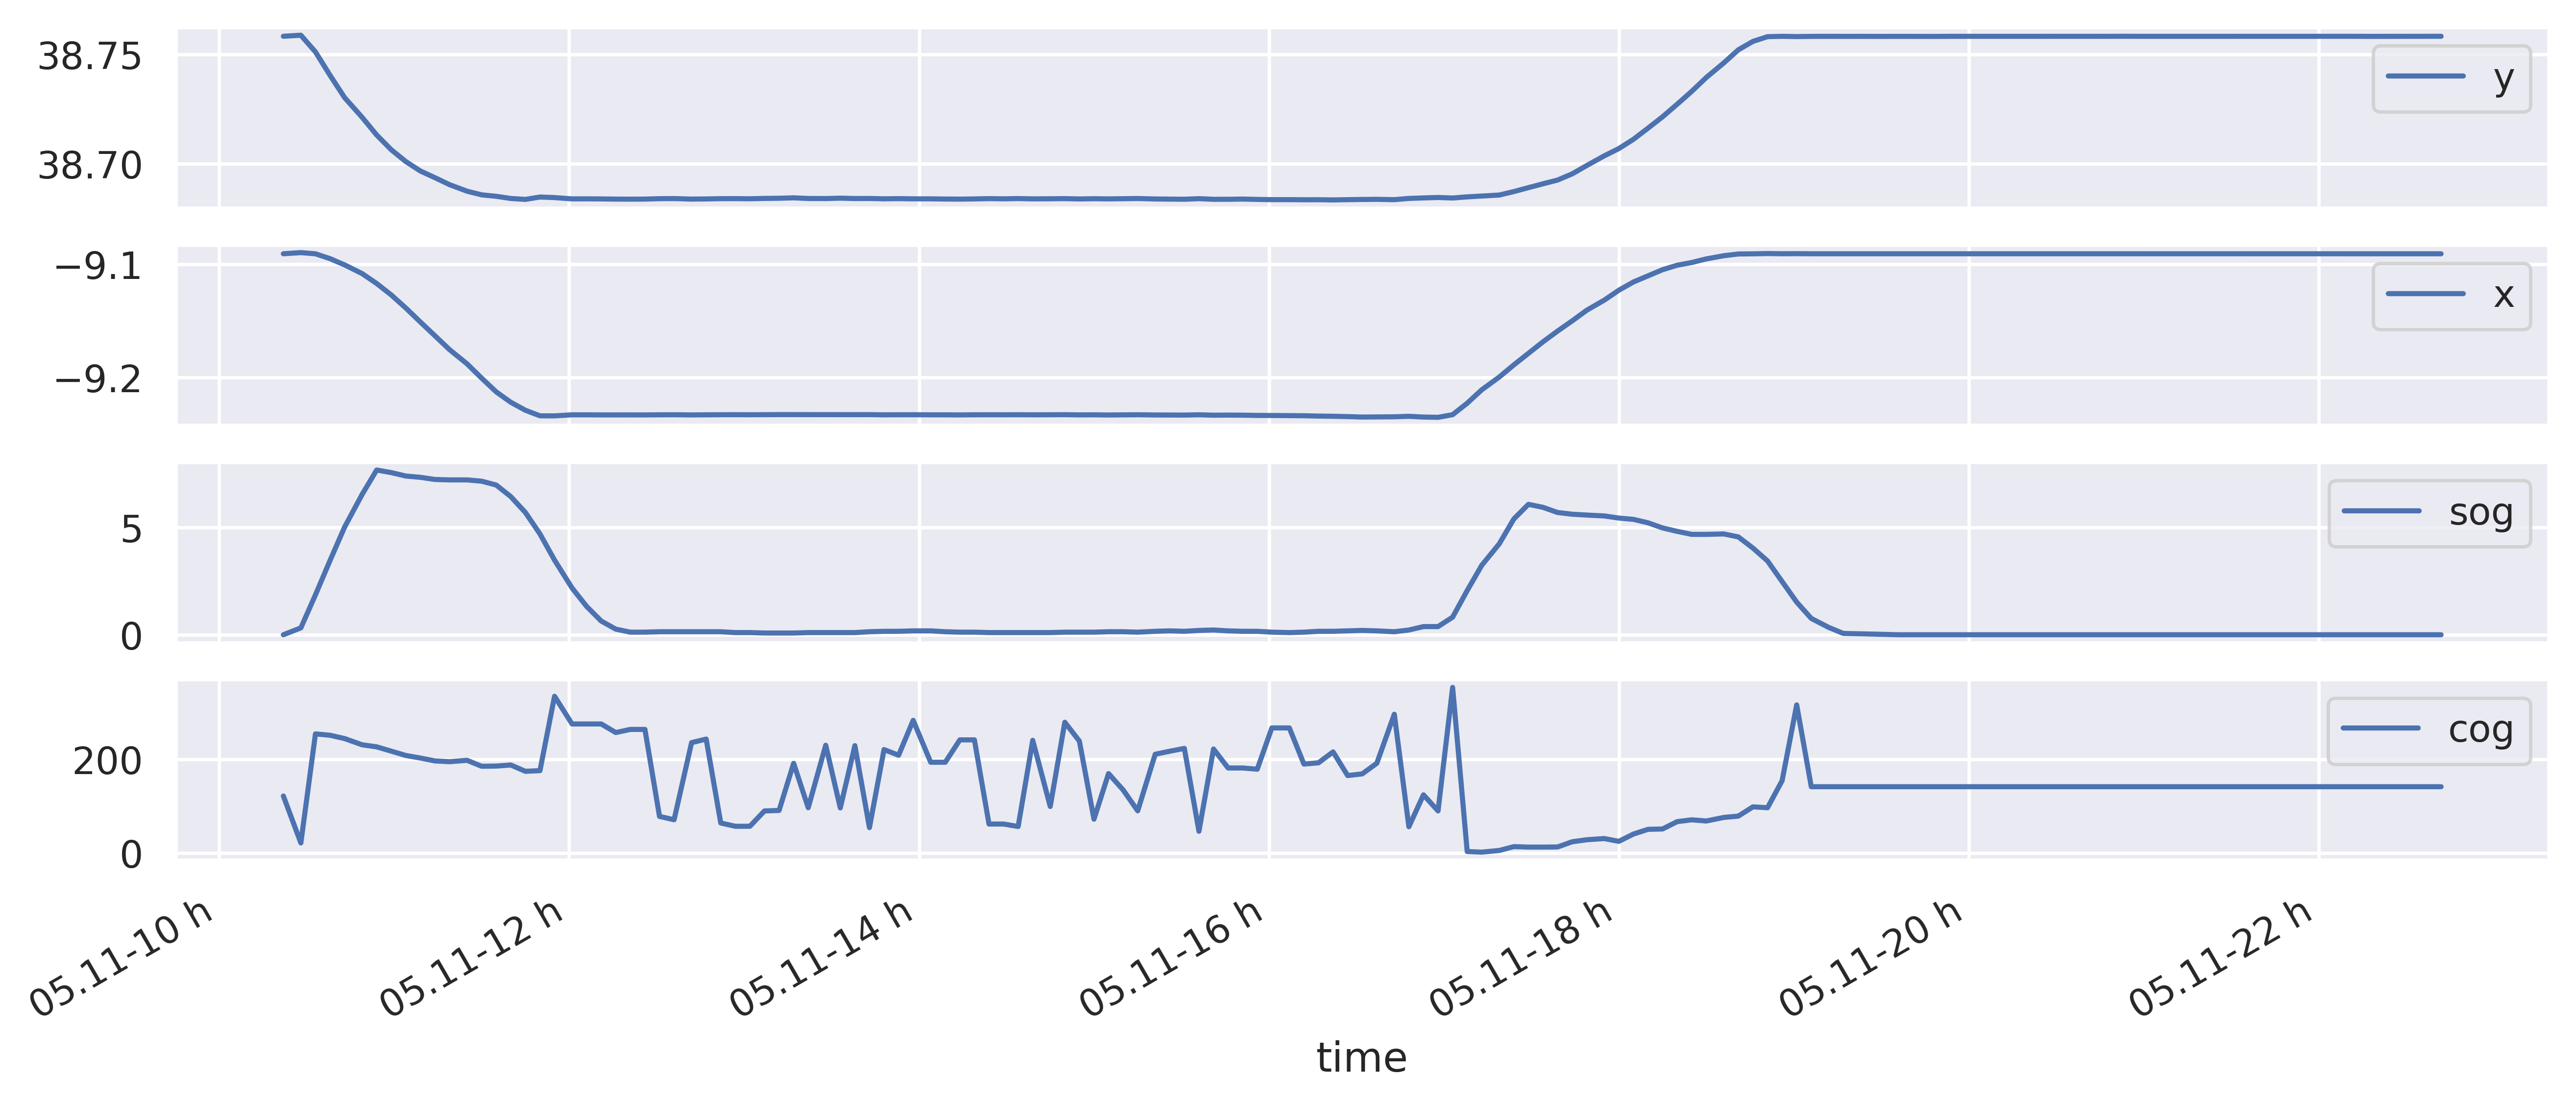
\includegraphics[scale = .5]{figures/Ch3/ts_example.png}
    \caption{Trajectory represented in Fig.X, presented as a Multivariate Time Series.}
    \label{fig: MTimeSeries_example}
\end{figure}

\todo[inline]{Needs Intro for this section...}


\section{Anomaly Detection Service}
\subsection{Vessel Rendezvous}
A requirement imposed by the MARISA project, was the development of services, able to detect and generate alarms when two or more vessels are approaching close to each other. This in the maritime world can be called as rendezvous.

The concept of rendezvous in the Maritime world is quite complex, as there are numerous legislation. For the purpose of this work, and because the emphasis is on the alarm generation of possible rendezvous, a simplification of this definition is assumed, therefore: 

~\textbf{Vessel Rendezvous}, for this work is considered as the interception or closeness of two or more vessels, in a configurable time period.

An algorithm was developed in which the a distance ~\textbf{d}, is given as a parameter. For every single Vessel Track, the track is partitioned into time-groups(e.g. a time-group of 5min), ~\textbf{t}, defined also as a parameter. If two or more Vessels, are in the same ~\textbf{t} with a distance smaller than ~\textbf{d}, an alarm is generated for those two vessels.

Figure~\ref{fig: VesselRendevouz2d}, shows two different Vessel Routes, with the axis representing the X and Y coordinate, respectively.

\begin{figure}[H]
	\centering
	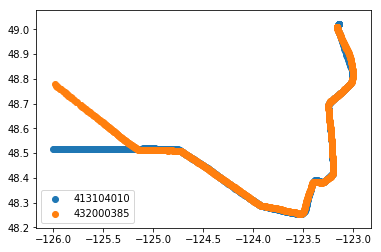
\includegraphics[scale = .8]{figures/VesselRendevouz2d}
    \caption{Two vessel routes}
    \label{fig: VesselRendevouz2d}
\end{figure}

While is obvious that the routes are similar in a positional way, they occur at different times, as is can be see in the figure ~\ref{fig: VesselRendevouz3d} .

\begin{figure}[H]
	\centering
	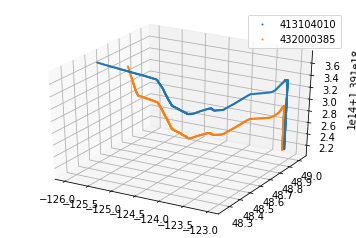
\includegraphics[scale = .9]{figures/VesselRendevouz3d}
    \caption{Two vessel routes, time on Z-axis}
    \label{fig: VesselRendevouz3d}
\end{figure}


\subsection{Navigational Status Validation}
AIS Navigational Status describes the Vessel current navigational activity based on a set static set of defined Status, as shown in Table XX. The Navigational Status needs to be manually set and constantly updated (according to the current Vessel activity), by the Vessel crew members. The problem with relying on Human action to update the actual Vessel Navigational Status is that is really prone to errors. 

\begin{table}[H]
\centering
\caption{My caption}
\label{Table: AIS Status}
\begin{tabular}{@{}cl@{}}
\toprule
\begin{tabular}[c]{@{}c@{}}Navigational \\ Status Value\end{tabular} & \multicolumn{1}{c}{Description} \\ \midrule
0 & under way using engine \\
1 & at anchor \\
2 & not under command \\
3 & restricted maneuverability \\
4 & constrained by draught \\
5 & moored \\
6 & aground \\
7 & engaged in fishing \\
8 & under way sailing \\
9 - 14 & reserved for future use \\
15 & Default \\ \bottomrule
\end{tabular}
\end{table}

Our approach towards the detection of the miss-use Navigational Status, started by firstly analyzing what each Navigational Status was used for. Then we analyzed the frequency of which was used. We concluded, based on the frequency count of each Status that there are AIS Status which are solely used in special scenarios. Thus, for this work we focus on the detection and validation of AIS Status that can be justified on the Vessels Dynamic Features.

\missingfigure{COUNT PLOT - AIS STATUS COUNTS}

With the help of Maritime Officers Expertise, we enriched our Description from each Navigational Status, be classifying the appropriate Stopped or Moving Label to each Navigational Status based on the the Kinematics it presents, as it is shown in Table XX.

By determining based on the reported AIS kinematic features, if a Vessel is in fact Stopped or Moving as it is demonstrated in Section XX. By comparing the compared reported Navigational Status agains what was the Kinematic  

We effectively detect the Vessels AIS messages that are reported with the wrong AIS Navigational Status. For every Vessel with wrong (generate an anomaly)...


apriori determining for each AIS message, based on the reported kinematic features, if it is Moving or Stopped. We can 

determining the actual kinematics characteristics of a Vessel

and represent little occurrences on the global count of the Data-Set.

as it is represented in Fig

being considered Anomalous, our approach towards the detection of this  

\subsection{Fishing Activity Detection}
Based on the xxx presented in the Sections above, we decided in order to enrich the functionalities of the Navigational Status Detection, to detecting Fishing Activity from Fishing Vessels. Vessel Fishing activity is commonly defined as the period of time when the Vessel has the fishing gear on the water. Although for the purpose of this work, and as we currently didn't had access to any Classified Data-Sets that allowed the development of this task in a Supervised Manner, we decided to generalize the definition of Fishing Activity to the activity which could be detected based on Vessels kinematic information, which induce the Vessels activity of Fishing. 

To tackle this problem, we firstly analyzed the the kinematic feature that better describes the Fishing activity which is the Vessel Speed (SOG). As Vess


In order to detect the Fishing activitie we focused on the detection 
To tackle, the detection of Fishing, So, the main objective of this  


to be a no precise manner to in-fact know if a Vessel was fishing or not, with the fishing gear in the water at a certain point, we define Fishing as the possible Kinematic generalization it can represent.





can be defined in many different ways, but for the porpouse of this work, we consied Fishing by the 
The detection of Fishing Activity, for this work is done, by estimating the fishing probability, for each point reported by an AIS Fishing Vessel. 

is focused on the point based probability estimation of the probability that the estimation 

To the best of our knowledge, there are no Classified Data-Sets that allow the development of this task to be a 

Fishing can be defined in many different ways, as we were soon to realize that there are enoumerous diferente tech

but for the purpose of this work, define fishing as the time-period when a Vessel is engaged in the activitie by having the fishing gear 

By knowing anyting apriory of a Vessel Trajectory, we clu



